\section{Conclusions}
The current implementation is quite good-working, and can keep a small object floating for up to some minutes if the object is carefully positioned in order to minimize oscillations. A good control for about one minute can be reached without caring too much about initial positioning. Some interesting facts and possible defects have been noticed after fabricating the circuit:

\begin{itemize}
\item{The control is more stable if the amplifier stage is bypassed and only the ADC protection net is kept. This is probably due to the fact that the amplifier's gain is quite low (1.3) and thus does not increase very much the readings' accuracy. On the other hand, the amplifier stage adds some noise which increases oscillations after a little time and produce instability into the control;}
\item{Being a simple P controller, the object is not positioned precisely in space, its position depending mostly on its weight. Anyway, increasing and decreasing its position works as expected. A finer control algorithm could solve this problem (due to the integral error of the controller), and could for sure also damp the noise due to the amplifier, making it an advantageous insertion again;}
\item{The coil is seldom fully active. Thus, decreasing the main supply voltage to 9V with a linear regulator could help having a cleaner supply without the need of bulky $1000\mu F$ capacitors, while keeping the levitation system work as excepted. Also, this would reduce a lot the power dissipation on the other voltage regulators and thus reduce heat;}
\item{Some rails on the printed circuit board have been designed in a non-savy way in order to reduce the total area of the board. A bigger PCB would have helped in having a cleaner routing and less broken/short-circuited tracks when soldering;}
\item{The sensor's cable is a simple 3-wires, 3-pins cable. As this cable is positioned very near to the mouse interface cable, better shielding should probably have been done. In fact, when pressing one of the buttons of the mouse, a small fluctuation of the read magnetic field can be observed from the PC interface, although it is not clear whether it is big and long-lasting enough to influence the control.}
\end{itemize}

\begin{figure}[htbp]
\centering
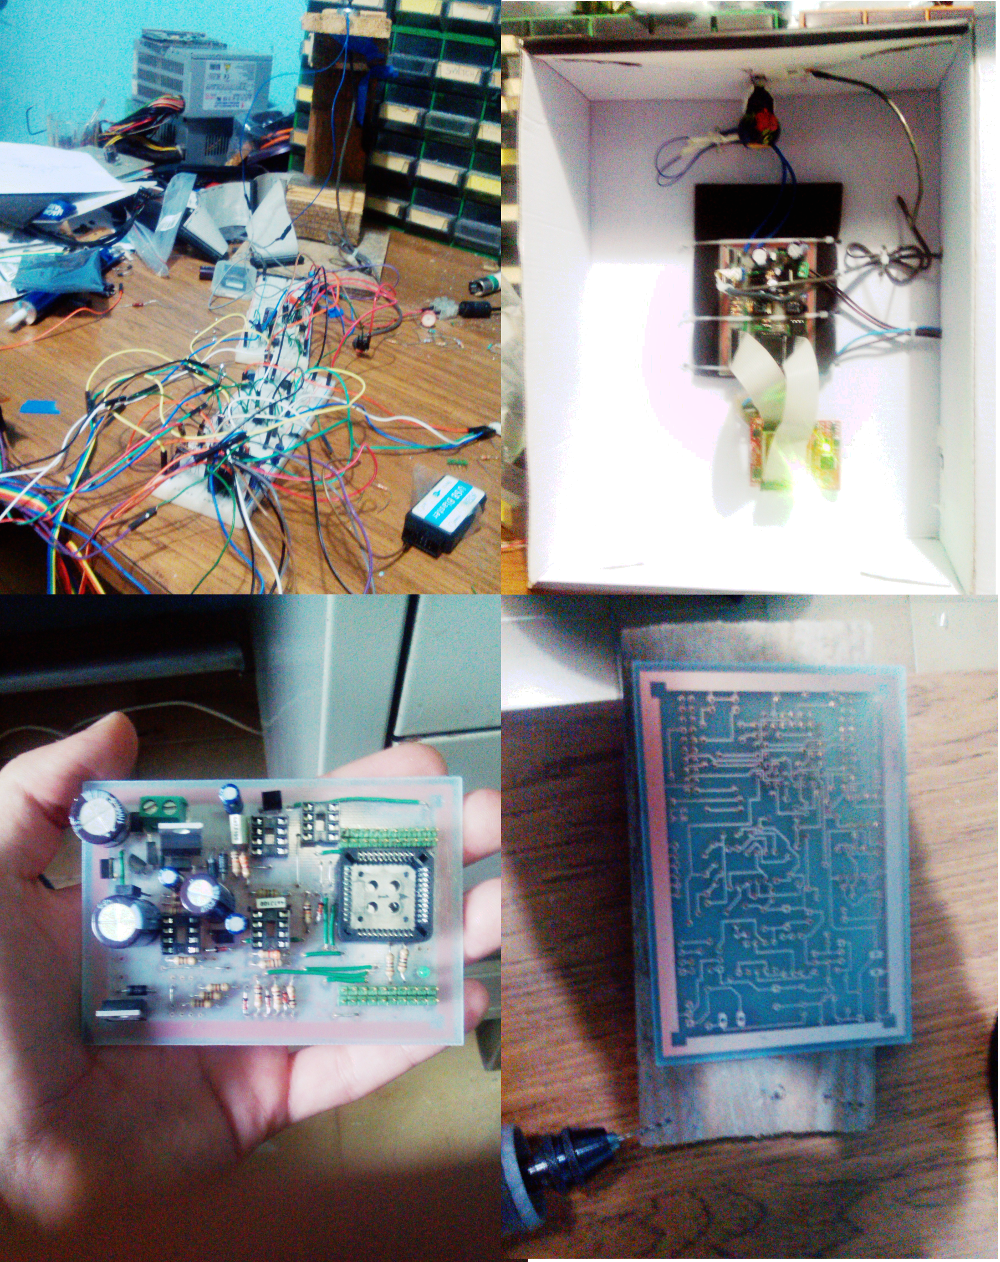
\includegraphics[width=4in]{Graphics/mosaic}
\caption{Some photos taken during various project's stages. From top-left corner: status of the first working prototype; final implementation levitating a small toy doll; final PCB after printing; final main circuit board.}
\end{figure}
